%!TEX root = ../thesis.tex

\chapter[benchmarking generative latent variable models for speech]{Benchmarking Generative Latent Variable Models for Speech}
\label{chp:paper-benchmarking}

\textit{This chapter is a piece of original research published as part of the project:} \newline
\begin{center}
    \begin{enumerate}[leftmargin=8mm,rightmargin=8mm,topsep=0mm,label={[\Alph*]}]
        \setcounter{enumi}{3}
        \item \fullcite{havtorn_benchmarking_2022} \main \hspace{0.1em} \parencite{havtorn_benchmarking_2022}
        \end{enumerate}
\end{center}

\ifthenelse{\equal{\skippapers}{true}}{}{


\section{Abstract}
Stochastic latent variable models (LVMs) achieve state-of-the-art performance on natural image generation but are still inferior to deterministic models on speech. In this paper, we develop a speech benchmark of popular temporal LVMs and compare them against state-of-the-art deterministic models. We report the likelihood, which is a much used metric in the image domain, but rarely, or incomparably, reported for speech models. To assess the quality of the learned representations, we also compare their usefulness for phoneme recognition. Finally, we adapt the Clockwork VAE, a state-of-the-art temporal LVM for video generation, to the speech domain. Despite being autoregressive only in latent space, we find that the Clockwork VAE can outperform previous LVMs and reduce the gap to deterministic models by using a hierarchy of latent variables.


\section{Introduction}
After the introduction of the variational autoencoder (VAE,  \textcite{kingma_autoencoding_2014, rezende_stochastic_2014}) quickly came two temporal extensions for modeling speech data \parencite{chung_recurrent_2015, fraccaro_sequential_2016}. Since then, temporal LVMs have undergone little development compared to their counterparts in the image domain, where LVMs recently showed superior performance to autoregressive models such as PixelCNN \parencite{oord_pixel_2016, oord_conditional_2016, salimans_pixelcnn_2017}. The improvements in the image domain have been driven mainly by top-down inference models and deeper latent hierarchies \parencite{sonderby_ladder_2016, maaloe_biva_2019, vahdat_nvae_2020, child_very_2021,sinha_consistency_2021,kingma_variational_2021}. In speech modeling however, autoregressive models such as the WaveNet remain state-of-the-art \parencite{oord_wavenet_2016}.

To compare and develop LVMs for speech, we need good benchmarks similar to those in the image domain. Image benchmarks commonly compare likelihood scores, but research in the speech domain often omits reporting a likelihood \parencite{oord_wavenet_2016, hsu_unsupervised_2017, oord_neural_2018} or report likelihoods that are incomparable due to subtle differences in the assumed data distribution \parencite{chung_recurrent_2015, fraccaro_sequential_2016, hsu_unsupervised_2017, aksan_stcn_2019}. Without a proper standard, it is difficult to compare explicit likelihood models for speech and develop them in an informed manner.

To advance the state of LVMs for speech, this paper (i) develops a benchmark for LVMs based on model likelihood, (ii) introduces a hierarchical LVM architecture without autoregressive decoder, (iii) compares LVMs to deterministic counterparts including WaveNet, and (iv) qualitatively and quantitatively evaluates the latent variables learned by different LVMs based on their usefulness for phoneme recognition. We find that:
\begin{itemize}[leftmargin=8mm]
    \setlength\itemsep{-0em}
    \item [(I)] State-of-the-art LVMs achieve likelihoods that are inferior to WaveNet at high temporal resolution but are superior at lower resolutions. Interestingly, we find that a standard LSTM \parencite{hochreiter_long_1997} almost matches the likelihood of WaveNet.
    \item [(II)] LVMs with powerful autoregressive decoders achieve better likelihoods than the non"=autoregressive LVM.
    \item[(III)] The expressiveness of LVMs for speech increases with a deeper hierarchy of stochastic latent variables, similar to conclusions within image modeling. % \parencite{maaloe_biva_2019, vahdat_nvae_2020, child_very_2021}.
    \item[(IV)] LVMs learn rich representations that are as good or better than Mel spectrograms for phoneme recognition also when using only 10 minutes of labeled data.
\end{itemize}
At a high level, this benchmark brings order to LVM model comparisons for speech and also provides useful reference implementations of the models.\footnote{\href{https://github.com/JakobHavtorn/benchmarking-lvms}{\url{github.com/JakobHavtorn/benchmarking-lvms}}} 
% \footnote{\fontsize{8.5}{0}\selectfont\texttt{ \url{github.com/anonymous/available-later}}}.
Before presenting the results, we provide a brief survey of existing LVMs for speech in a coherent notation. 


\section{Latent variable models for speech}
\begin{figure*}[t]
    \centering
    \begin{multicols}{5}
        \resizebox{!}{0.18\paperheight}{
            \begin{tikzpicture}
                \node[obs] (x_t) {$\xb_t$};
                
                % \node[above=0.75cm of x_t, xshift=0cm] (cap1) {$p(\xb_t|\xb_{<t})$};
                \node[above=0.4cm of x_t] (caption) {LSTM};
                
                \node[det,below=2.55cm of x_t] (d_t) {$\db_{t}$};
                \node[det,left=0.75cm of d_t] (d_tm1) {$\db_{t-1}$};
                \node[obs,below=0.75cm of d_t] (x_tm1) {$\xb_{t-1}$};
                
                \edge[deterministic-skip-color]{x_tm1}{d_t};
                \edge[deterministic-skip-color]{d_t}{x_t};
                \edge[deterministic-skip-color]{d_tm1}{d_t};
                \edge[draw=white,bend right]{d_t}{x_t};  % for identical width to others
            \end{tikzpicture}
        }
        \\
        \resizebox{!}{0.18\paperheight}{
            \begin{tikzpicture}
                \node[obs] (x_t) {$\xb_t$};
                
                % \node[above=0.75cm of x_t, xshift=0cm] (cap1) {$p(\xb_t|\zb_{\leq t},\xb_{<t}) p(\zb_t|\xb_{<t},\zb_{<t})$};
                \node[above=0.4cm of x_t] (caption) {VRNN};
                
                \node[latent,below=0.75cm of x_t] (z_t) {$\zb_t$};
                \node[latent,left=0.75cm of z_t] (z_tm1) {$\zb_{t-1}$};
                
                \node[det,below=0.75cm of z_t] (d_t) {$ b_{t}$};
                \node[det,below=0.75cm of z_tm1] (d_tm1) {$\db_{t-1}$};
                \node[obs,below=0.75cm of d_t] (x_tm1) {$\xb_{t-1}$};
                
                \edge[deterministic-skip-color]{x_tm1}{d_t};
                \edge[]{d_t}{z_t};
                \edge[]{z_tm1}{d_t};
                \edge[deterministic-skip-color]{d_tm1}{d_t};
                \edge[]{z_t}{x_t};
                \edge[deterministic-skip-color,bend right]{d_t}{x_t};
            \end{tikzpicture}
        }
        \\
        \resizebox{!}{0.18\paperheight}{
            \begin{tikzpicture}
                \node[obs] (x_t) {$\xb_t$};
                
                % \node[above=0.75cm of x_t, xshift=0cm] (cap1) {$p(\xb_t|\zb_{\leq t},\xb_{<t}) p(\zb_t|\xb_{<t},\zb_{<t})$};
                \node[above=0.4cm of x_t] (caption) {SRNN};
                
                \node[latent,below=0.75cm of x_t] (z_t) {$\zb_t$};
                \node[latent,left=0.75cm of z_t] (z_tm1) {$\zb_{t-1}$};

                \node[det,below=0.75cm of z_t] (d_t) {$\db_{t}$};
                \node[det,below=0.75cm of z_tm1] (d_tm1) {$\db_{t-1}$};
                \node[obs,below=0.75cm of d_t] (x_tm1) {$\xb_{t-1}$};
                
                \edge[deterministic-skip-color]{x_tm1}{d_t};
                \edge[]{d_t}{z_t};
                \edge[]{z_tm1}{z_t};
                \edge[deterministic-skip-color]{d_tm1}{d_t};
                \edge[]{z_t}{x_t};
                \edge[deterministic-skip-color,bend right]{d_t}{x_t};
            \end{tikzpicture}
        }
        \\
        \resizebox{!}{0.18\paperheight}{
            \begin{tikzpicture}
                \node[obs] (x_t) {$\xb_t$};
                % \node[above=0.75cm of x_t, xshift=0cm] (cap1) {$p(\xb_t|\zb_t,\xb_{t-r:t-1})$};
                \node[above=0.4cm of x_t] (caption) {STCN};
                
                \node[latent,below=0.75cm of x_t] (z_t) {$\zb_t$};
                \node[left=0.025cm of z_t] (dots) {$\cdots$};
                \node[latent,left=0.75cm of z_t] (z_tmr) {$\zb_{t-r'}$};
                
                \node[det,below=0.75cm of z_t] (d_t) {$\db_{t}$};
                \node[obs,below=0.75cm of d_t] (x_tm1) {$\xb_{t-1}$};
                \node[left=0.025cm of x_tm1] (dots) {$\cdots$};
                \node[obs,left=0.75cm of x_tm1] (x_tmr) {$\xb_{t-r}$};
                
                \edge[]{x_tm1}{d_t};
                \edge[]{x_tmr}{d_t};
                \edge[]{d_t}{z_t};
                \edge[]{z_t}{x_t};
                \edge[]{z_tmr}{x_t};
                \edge[draw=white,bend right]{d_t}{x_t};  % for identical width to others 
            \end{tikzpicture}
        }
        \\
        \resizebox{!}{0.18\paperheight}{
            \begin{tikzpicture}
                \node[obs] (x_t) {$\xb_t$};%
                
                % \node[above=0.75cm of x_t, xshift=0cm] (cap1) {$p(\xb_t|\zb_{\leq t}) p(\zb_t|\zb_{<t})$};
                \node[above=0.4cm of x_t] (caption) {CW-VAE};
                
                \node[latent,below=0.75cm of x_t] (z_t) {$\zb_t$};
                \node[latent,left=0.75cm of z_t] (z_tm1) {$\zb_{t-1}$};
                
                \node[det,below=0.75cm of z_t] (d_t) {$\db_{t}$};
                \node[det,below=0.75cm of z_tm1] (d_tm1) {$\db_{t-1}$};
                \node[obs,below=0.75cm of d_t,draw=white,fill=white] (x_tm1) {};
                
                \edge[]{d_t}{z_t};
                \edge[bend right]{d_t}{x_t};
                \edge[]{z_tm1}{d_t};
                \edge[]{d_tm1}{d_t};
                \edge[]{z_t}{x_t};
            \end{tikzpicture}
        }
        \end{multicols}
    \caption[Generative models for an LSTM, the VRNN, SRNN, STCN, and CW-VAE models.]{
        Generative models for a single timestep of a deterministic autoregressive LSTM, the VRNN and SRNN as well as the STCN and CW-VAE both with a single layer of latent variables. 
        Red arrows indicate purely deterministic paths from the output $\xb_t$ to previous input $\xb_{<t}$ without passing a stochastic node. 
        The models differ in their use of latent variables and dependencies especially autoregressive dependencies and skip connections. 
        % In an LSTM, information flows deterministically from previous observed variables to the next. 
        % The VRNN and SRNN use stochastic latent variables but also include deterministic skip connections from previous observed variables. 
        % The STCN is also autoregressive in $\xb$ but does not use deterministic skip connections from $\xb_{t-1}$ to $\xb_t$. 
        % The CW-VAE is not autoregressive on the observed variable which forces information to flow through the latent variables. 
        We provide more elaborate graphical illustrations including inference models in \cref{fig: clockwork vae inference generative models 2 layered} and appendix~\cref{app: additional graphical models}.
        }
    \label{fig: autoregressive vrnn srnn cwvae 1L graphs}
\end{figure*}


% \linepenalty=1000
% \subsection{Related work}
LVMs formulated as VAEs continue to be of interest since they are able to learn an approximation to the posterior distribution of assumed latent variables. The posterior is usually of a reduced dimensionality compared to the input and lies close to a known prior distribution. Approximate posteriors have various applications e.g. semi"=supervised learning \parencite{kingma_semi-supervised_2014} and anomaly detection \parencite{havtorn_hierarchical_2021}.

In recent years, several complementary methods have been proposed to improve the expressiveness of VAEs. These include building more expressive priors via methods such as normalizing flows \parencite{rezende_variational_2015} and building a deeper hierarchy of stochastic latent variables such as the Ladder VAE \parencite{sonderby_ladder_2016}. In this research, we focus on the latter due to the recent breakthroughs in image modeling using VAEs without costly autoregressive dependencies on the observed variable \parencite{maaloe_biva_2019,vahdat_nvae_2020,child_very_2021}.

Several works have applied LVMs to speech. Among the first contributions were the VRNN \parencite{chung_recurrent_2015} and SRNN \parencite{fraccaro_sequential_2016} which can be seen as conditional VAEs per timestep. Other recent LVMs include the FH-VAE \parencite{hsu_unsupervised_2017}, which leverages an additional latent variable to capture global features, and Z-forcing \parencite{goyal_zforcing_2017}, which resembles the SRNN but includes an auxiliary task in the latent space to increase its utilization. The VQ-VAE \parencite{oord_neural_2018} is a hybrid between an LVM and an autoregressive model which uses a quantized latent space to improve the quality of generated samples. The Stochastic WaveNet \parencite{lai_stochastic_2018} and STCN \parencite{aksan_stcn_2019} use WaveNet encoder and decoders and temporally independent latent variables.

In this paper, we focus on the VRNN, SRNN and STCN. We exclude the Stochastic WaveNet as it is similar to STCN and achieves inferior likelihoods \parencite{aksan_stcn_2019}. The FH-VAE, with disjoint latent variables and discriminative objective, Z-forcing, with an auxiliary task, and the VQ-VAE, with a quantized latent space and autoregressive prior fitted after training, all introduce significant changes to the original VAE framework and are also not included here.

All selected models have autoregressive generative models which let future observed variables be generated by conditioning on previously generated values. Inspired by recent progress in the image domain, we therefore formulate and benchmark a novel temporal LVM which does not rely on an autoregressive decoder. We do so by adapting the hierarchical Clockwork Variational Autoencoder \parencite{saxena_clockwork_2021}, originally proposed for video generation, to speech.


\subsection{Sequential deep latent variable models}
The selected models are all sequential deep latent variable models trained with variational inference and the reparameterization trick \parencite{kingma_autoencoding_2014}.
% The VRNN, SRNN, STCN and CW-VAE are all autoencoders trained with variational inference and the reparameterization trick \parencite{kingma_autoencoding_2014}. 
They take as input a variable-length sequence $\xb_{1:T} = \left(\xb_1, \xb_2, \dots, \xb_{T}\right)$ with $\xb_t \in \mathbb{R}^{D_x}$. 
% The VRNN, SRNN, STCN and CW-VAE are all VAEs \parencite{kingma_autoencoding_2014} that take as input a variable-length sequence $\xb_{1:T} = \left(\xb_1, \xb_2, \dots, \xb_{T}\right)$ with $\xb_t \in \mathbb{R}^{D_x}$. 
We let $\xb_{1:T}$ refer to the observed variable or a downsampled version of it. We will sometimes use $\xb$ to refer to the sequence $\xb_{1:T}$ when it is not ambiguous.
% In general, $\xb_{1:T}$ may refer to the original observed variable or a deterministically downsampled representation of the observed variable. We will sometimes use $\xb$ to refer to the full sequence $\xb_{1:T}$ when it is not ambiguous.

First, $\xb_{1:T}$ is encoded to a temporal stochastic latent representation $\zb_{1:T} = \left( \zb_1, \zb_2, \dots, \zb_{T} \right)$ with $\zb_t\in \mathbb{R}^{D_z}$. This representation is then used to reconstruct the original input $\xb_{1:T}$.
The latent variable is assumed to follow some prior distribution $p(\zb_t|\cdot)$ where the dot indicates that it may depend on latent and observed variables at previous timesteps, $\zb_{<t}$ and $\xb_{<t}$ where $\zb_{<t} := \left( \zb_1, \zb_2, \dots, \zb_{t-1} \right)$. 

The models are trained to maximize a likelihood objective. The exact marginal likelihood $\log p_\thetab(\xb)$, where $\thetab$ are parameters of the generative model, is intractable to optimize due to the integration over the latent space. Instead, we introduce the variational approximation $q_\phib(\zb|\xb)$ to the true posterior. Via Jensen's inequality this yields the well-known evidence lower bound (ELBO) on the exact likelihood $\mathcal{L}(\thetab,\phib;\xb)$
which can be jointly optimized with respect to  $\{\thetab, \phib\}$ using stochastic gradient descent methods. We omit the $\thetab$ and $\phib$ subscripts for the remainder of the paper.
\begin{equation}
    \log p_\thetab(\xb) = \log \int p_\thetab(\xb,\zb) \, \mathrm{d}\zb  \geq \mathbb{E}_{q_\phib(\zb|\xb)} \left[ \log \frac{p_\thetab(\xb,\zb)}{q_\phib(\zb|\xb)} \right] =: \mathcal{L}(\thetab,\phib;\xb) \label{eq: elbo} \enspace,
\end{equation}
Graphical illustrations of the models can be seen in \cref{fig: autoregressive vrnn srnn cwvae 1L graphs} with more illustrations in appendix~\cref{app: additional graphical models}.


\subsection{Variational recurrent neural network ({\small VRNN})}
The VRNN \parencite{chung_recurrent_2015} is essentially a VAE per timestep. At timestep $t$, the VAE is conditioned on the hidden state of a recurrent neural network (RNN), $\db_{t}\in\mathbb{R}^{D_d}$, with state transition $\db_{t} = f([\xb_{t-1}, \zb_{t-1}], \db_{t-1})$ where $[\cdot, \cdot]$ denotes concatenation. 
The VRNN uses a Gated Recurrent Unit (GRU, \textcite{cho_properties_2014}) for $f$.
The joint distribution factorizes over time and the latent variables are autoregressive in both the observed and latent space,
\begin{equation}
    p(\xb_{1:T},\zb_{1:T}) = \prod_{t=1}^{T} p(\xb_t|\xb_{<t},\zb_{\leq t}) p(\zb_t|\xb_{<t},\zb_{<t}) \enspace . \label{eq: vrnn joint factorization}
\end{equation}
The approximate posterior similarly factorizes over time,
\begin{equation}
    q(\zb_{1:T}|\xb_{1:T}) = \prod_{t=1}^{T} q(\zb_t|\xb_{\leq t},\zb_{<t}) \enspace . \label{eq: vrnn inference factorization}
\end{equation}
From this, the ELBO for the VRNN is
\begin{equation}
    \mathcal{L}(\xb) = ~ \mathbb{E}_{q(\zb_{1:T}|\xb_{1:T})} \bigg[ \sum_{t} \log p(\xb_t|\xb_{<t},\zb_{\leq t}) - D_\text{KL}\left( q(\zb_t|\xb_{\leq t},\zb_{<t}) \parallel p(\zb_t|\xb_{<t},\zb_{<t}) \right)  \bigg] \label{eq: vrnn elbo} \enspace .
\end{equation}
% \begin{equation}
% \begin{split}
%     \mathcal{L}(\xb) =&~ \mathbb{E}_{q(\zb_{1:T}|\xb_{1:T})} \bigg[ \sum_{t} \log p(\xb_t|\xb_{<t},\zb_{\leq t}) \\ & - \text{KL}\left( q(\zb_t|\xb_{\leq t},\zb_{<t}) \parallel p(\zb_t|\xb_{<t},\zb_{<t}) \right)  \bigg] \enspace .
%     \label{eq: vrnn elbo}
% \end{split}
% \end{equation}
The VRNN uses diagonal covariance Gaussian distributions $\mathcal{N}$ for the prior and posterior distributions. We denote the output distribution of choice by $\mathcal{D}$. 
% \begin{align}
%     q(\zb_t|\xb_{\leq t},\zb_{<t}) &= \mathcal{N}\left(\alphab_{q}(\xb_{t},\db_{t})\right) \label{eq: vrnn parameterization inference} \\
%     p(\zb_t|\xb_{<t},\zb_{<t}) &= \mathcal{N}\left(\alphab_{p}(\db_t)\right) \label{eq: vrnn parameterization prior} \\
%     p(\xb_t|\xb_{<t},\zb_{\leq t}) &= \mathcal{D}\left(\betab(\zb_{t},\db_{t})\right) \enspace . \label{eq: vrnn parameterization observation}
% \end{align}
\begin{gather}
    p(\zb_t|\xb_{<t},\zb_{<t}) = \mathcal{N}\left(\alphab_{p}(\db_t)\right) \enspace , \nonumber \\
    p(\xb_t|\xb_{<t},\zb_{\leq t}) = \mathcal{D}\left(\betab(\zb_{t},\db_{t})\right) \enspace , \label{eq: vrnn parameterization generative} \\
    q(\zb_t|\xb_{\leq t},\zb_{<t}) = \mathcal{N}\left(\alphab_{q}(\xb_{t},\db_{t})\right) \enspace . \nonumber 
    \label{eq: vrnn parameterization inference}
\end{gather}
All sets of distributional parameters, $\alphab_q,\alphab_p$ and $\betab$, are the outputs of densely connected neural networks which we notationally overload as functions in equations~\cref{eq: vrnn parameterization generative} and \cref{eq: vrnn parameterization inference}. It is common to refer to $\alphab_q$ as the inference model or encoder and $\betab$ as the decoder. Together with $\betab$, the structural model $\alphab_p$ forms the generative model.

Since the decoder is dependent on $\db_t$, the transition function $f$ allows the VRNN to learn to ignore parts of or the entire latent variable and establish a purely deterministic transition from $\xb_{t-1}$ to $\db_t$ (\cref{fig: autoregressive vrnn srnn cwvae 1L graphs}). This failure mode is commonly referred to as posterior collapse and is a well-known weakness of VAEs with powerful decoders \parencite{bowman_generating_2016, sonderby_ladder_2016}.


\subsection{Stochastic recurrent neural network ({\small SRNN})}
The SRNN \parencite{fraccaro_sequential_2016} is similar to the VRNN but differs by separating the stochastic latent variables from the deterministic representations (\cref{fig: autoregressive vrnn srnn cwvae 1L graphs}). That is, the GRU state transition is independent of $\zb_{1:T}$ such that $\db_{t} = f(\xb_{t-1}, \db_{t-1})$. With this, the joint $p(\xb_{1:T},\zb_{1:T})$ can be written as for the VRNN in \cref{eq: vrnn joint factorization}. The approximate posterior of $\zb_t$ is conditioned on the full observed sequence,
\begin{align}
    \label{eq: srnn inference factorization}
    q(\zb_{1:T}|\xb_{1:T}) = \prod_{t=1}^{T} q(\zb_t|\xb_{1:T},\zb_{t-1}) \enspace .
\end{align}
This is achieved by introducing a second GRU that runs backwards in time with transition $\ab_t = g([\xb_t,\db_t], \ab_{t+1})$. While $p(\xb_t|\xb_{<t},\zb_{\leq t})$ remains as in \cref{eq: vrnn parameterization generative}, we have
\begin{gather}
        p(\zb_t|\xb_{<t},\zb_{<t}) = \mathcal{N}\left(\alphab_{p}(\zb_{t-1},\db_t)\right) \enspace , \nonumber \\
        q(\zb_t|\xb_{1:T},\zb_{<t}) = \mathcal{N}\left(\alphab_{q}(\zb_{t-1},\ab_{t})\right) \enspace . \label{eq: srnn parameterization}
    % p(\xb_t|\xb_{<t},\zb_{\leq t}) &= \mathcal{D}\left(\vrho(\zb_{t},\db_{t})\right) \enspace . \label{eq: srnn parameterization observation}
\end{gather}
By inferring $\zb_t$ conditioned on the full sequence $\xb_{1:T}$, the SRNN performs smoothing. This has been noted to better approximate the true posterior of $\zb_t$ which can be shown to depend on the full observed sequence \parencite{bayer_mind_2021}. Comparatively, the VRNN performs filtering.


\begin{figure*}
    \centering
    % \h3ill
    \resizebox{!}{0.155\paperheight}{
        \begin{tikzpicture}
            % nodes
            \node[obs] (x_1) {$\xb_{t-3}$};
            \node[obs,right=.75cm of x_1] (x_2) {$\xb_{t-2}$};
            \node[obs,right=.75cm of x_2] (x_3) {$\xb_{t-1}$};
            \node[obs,right=.75cm of x_3] (x_4) {$\xb_{t}$};
            \node[obs,right=.75cm of x_4,fill=white,draw=white] (x_5) {$\dots$};

            \node[latent,above=.75cm of x_1](s_1_1){$\zb^{(1)}_{t-3}$};
            \node[latent,above=.75cm of x_2](s_1_2){$\zb^{(1)}_{t-2}$};
            \node[latent,above=.75cm of x_3](s_1_3){$\zb^{(1)}_{t-1}$};
            \node[latent,above=.75cm of x_4](s_1_4){$\zb^{(1)}_{t}$};
            \node[latent,above=.75cm of x_5,fill=white,draw=white](s_1_5){$\dots$};

            \node[latent,above=.75cm of s_1_1](s_2_1){$\zb^{(2)}_{t-3}$};
            \node[latent,above=.75cm of s_1_3](s_2_3){$\zb^{(2)}_{t-1}$};
            \node[latent,above=.75cm of s_1_5,fill=white,draw=white](s_2_5){$\dots$};

            % x to s first layer
            \edge[]{x_1}{s_1_1};
            \edge[]{x_2}{s_1_2};
            \edge[]{x_3}{s_1_3};
            \edge[]{x_4}{s_1_4};

            % x to s above layer
            \edge[bend left=40]{x_1}{s_2_1};
            \edge[]{x_2}{s_2_1};
            \edge[bend left=40]{x_3}{s_2_3};
            \edge[]{x_4}{s_2_3};

            % s per layer forward in time
            \edge[shared-function-color]{s_1_1}{s_1_2};
            \edge[shared-function-color]{s_1_2}{s_1_3};
            \edge[shared-function-color]{s_1_3}{s_1_4};
            \edge[shared-function-color]{s_1_4}{s_1_5};
            
            \edge[shared-function-color]{s_2_1}{s_2_3};
            \edge[shared-function-color]{s_2_3}{s_2_5};
            
            % s across layers on time
            \edge[shared-function-color]{s_2_1}{s_1_1};
            \edge[shared-function-color]{s_2_3}{s_1_3};

            % s across layers forward in time
            \edge[shared-function-color]{s_2_1}{s_1_2};
            \edge[shared-function-color]{s_2_3}{s_1_4};
            
            % \node[above=of s_2_1, yshift=-1.cm, xshift=2cm] (phi) {$q\pa{\zb_{1:T}^{(1:L)}|\xb_{1:T}}$};
            \node[above=of s_2_1, yshift=-0.5cm, xshift=2.5cm] (phi) {CW-VAE inference};
        \end{tikzpicture}
    }
    \hfill
    \resizebox{!}{0.155\paperheight}{
        \begin{tikzpicture}
            % nodes
            \node[obs] (x_1) {$\xb_{t-3}$};
            \node[obs,right=.75cm of x_1] (x_2) {$\xb_{t-2}$};
            \node[obs,right=.75cm of x_2] (x_3) {$\xb_{t-1}$};
            \node[obs,right=.75cm of x_3] (x_4) {$\xb_{t}$};
            \node[obs,right=.75cm of x_4,fill=white,draw=white] (x_5) {$\dots$};

            \node[latent,above=.75cm of x_1](s_1_1){$\zb^{(1)}_{t-3}$};
            \node[latent,above=.75cm of x_2](s_1_2){$\zb^{(1)}_{t-2}$};
            \node[latent,above=.75cm of x_3](s_1_3){$\zb^{(1)}_{t-1}$};
            \node[latent,above=.75cm of x_4](s_1_4){$\zb^{(1)}_{t}$};
            \node[latent,above=.75cm of x_5,fill=white,draw=white](s_1_5){$\dots$};

            \node[latent,above=.75cm of s_1_1](s_2_1){$\zb^{(2)}_{t-3}$};
            \node[latent,above=.75cm of s_1_3](s_2_3){$\zb^{(2)}_{t-1}$};
            \node[latent,above=.75cm of s_1_5,fill=white,draw=white](s_2_5){$\dots$};

            % x to s first layer
            \edge[]{s_1_1}{x_1};
            \edge[]{s_1_2}{x_2};
            \edge[]{s_1_3}{x_3};
            \edge[]{s_1_4}{x_4};

            % s per layer forward in time
            \edge[shared-function-color]{s_1_1}{s_1_2};
            \edge[shared-function-color]{s_1_2}{s_1_3};
            \edge[shared-function-color]{s_1_3}{s_1_4};
            \edge[shared-function-color]{s_1_4}{s_1_5};
            
            \edge[shared-function-color]{s_2_1}{s_2_3};
            \edge[shared-function-color]{s_2_3}{s_2_5};
            
            % s across layers on time
            \edge[shared-function-color]{s_2_1}{s_1_1};
            \edge[shared-function-color]{s_2_3}{s_1_3};
            
            % s across layers forward in time
            \edge[shared-function-color]{s_2_1}{s_1_2};
            \edge[shared-function-color]{s_2_3}{s_1_4};

            % \node[above=of s_2_1, yshift=-1.cm, xshift=2cm] (phi) {$p\pa{\xb_{1:T},\zb_{1:T}^{(1:L)}}$};
            \node[above=of s_2_1, yshift=-0.5cm, xshift=2.5cm] (phi) {CW-VAE generative};
        \end{tikzpicture}
    % \hfill
    }
\caption[Generative and inference models for a two-layered CW-VAE.]{
Inference (left) and generative (right) models for the CW-VAE with a hierarchy of $L=2$ latent variables, $s_1=1$ and $s_2=2$. 
The models are unrolled over four consecutive timesteps but note that the graph continues towards $t=0$ and $t=T$. 
Blue arrows indicate parameter sharing between inference and generative models. 
We omit the deterministic variable of \cref{fig: autoregressive vrnn srnn cwvae 1L graphs} for clarity.
}
\label{fig: clockwork vae inference generative models 2 layered}
\end{figure*}


\subsection{Stochastic temporal convolutional network ({\small STCN})}
The STCN \parencite{aksan_stcn_2019} is a hierarchical latent variable model with an autoregressive generative model based on WaveNet \parencite{oord_wavenet_2016}. Contrary to VRNN and SRNN, the latent variables have no transition functions connecting them over time.
Instead, a latent $\zb_t^{(l)}$ at layer $l$ is conditioned on a window of observed variables $\xb_{\scriptscriptstyle\mathcal{R}_t^{(l)}}$ via a WaveNet encoder where $\mathcal{R}_t^{(l)} = \cbra{t-r_l+1,\dots,t}$ and $r_l$ is the receptive field of the encoder at layer $l$. The window size grows exponentially with $l$.
\begin{equation}
    p(\xb_{1:T},\zb_{1:T}^{(1:L)}) = \prod_{t=1}^{T} p(\xb_t|\zb^{(1:L)}_{{\scriptscriptstyle \mathcal{R}}_{t}^{(1)}}) \prod_{l=1}^{L} p(\zb^{(l)}_{t}|\xb_{\scriptscriptstyle\mathcal{R}_{t-1}^{(l)}},\zb^{(l+1)}_{t}) \enspace , \nonumber
    \label{eq: stcn joint factorization}
\end{equation}
where $\zb_t^{(L+1)}:=\emptyset$ for notational convenience. 
The deterministic encoding is $\db_t^{(l)} = h(\xb_{\scriptscriptstyle\mathcal{R}_{t}^{(l)}})$ where $h$ is the encoder and $\db_t^{(l)}$ is extracted from the $l$'th layer similar to a Ladder VAE \parencite{sonderby_ladder_2016}. 
The approximate posterior is
\begin{equation}
    q\pa{\zb_{1:T}^{(1:L)}|\xb_{1:T}} = \prod_{t=1}^{T}\prod_{l=1}^{L} q\pa{\zb_{t}^{(l)}|\xb_{\scriptscriptstyle\mathcal{R}_{t}^{(l)}},\zb_t^{(l+1)}} \enspace .
\end{equation}
The factorized distributions are given as
% \begin{align}
%     q\left(\zb_t^{(l)}|\xb_{\scriptscriptstyle\mathcal{R}_{t}^{(l)}},\zb_t^{(l+1)}\right) &= \mathcal{N}\pa{\alphab_{q}^{(l)}\pa{\zb_t^{(l+1)},\db_t^{(l)}}} \enspace , \\
%     p\left(\zb_t^{(l)}|\xb_{\scriptscriptstyle\mathcal{R}_{t-1}^{(l)}},\zb_{t}^{(l+1)}\right) &= \mathcal{N}\pa{\alphab_{p}^{(l)}\pa{\zb_t^{(l+1)},\db_{t-1}^{(l)}}} \enspace \nonumber , \\
%     p\left(\xb_t|\zb^{(1:L)}_{\scriptscriptstyle\mathcal{R}_{t}^{(1)}}\right) &= \mathcal{D}\pa{\betab\pa{\zb^{(1:L)}_{\scriptscriptstyle\mathcal{R}_{t}^{(1)}}}} \enspace . \nonumber \label{eq: stcn parameterization} \\
% \end{align}
\begin{gather}
    p\left(\zb_t^{(l)}|\xb_{\scriptscriptstyle\mathcal{R}_{t-1}^{(l)}},\zb_{t}^{(l+1)}\right) = \mathcal{N}\pa{\alphab_{p}^{(l)}\pa{\zb_t^{(l+1)},\db_{t-1}^{(l)}}} \, \enspace , \nonumber \\
    p\left(\xb_t|\zb^{(1:L)}_{\scriptscriptstyle\mathcal{R}_{t}^{(1)}}\right) = \mathcal{D}\pa{\betab\pa{\zb^{(1:L)}_{\scriptscriptstyle\mathcal{R}_{t}^{(1)}}}} \enspace , \label{eq: stcn parameterization} \\
    q\left(\zb_t^{(l)}|\xb_{\scriptscriptstyle\mathcal{R}_{t}^{(l)}},\zb_t^{(l+1)}\right) = \mathcal{N}\pa{\alphab_{q}^{(l)}\pa{\zb_t^{(l+1)},\db_t^{(l)}}} \enspace . \nonumber
\end{gather}
The decoder $\betab\left(\zb^{(1:L)}_{\scriptscriptstyle\mathcal{R}_{t}^{(1)}}\right)$ is also a WaveNet. 


\subsection{Clockwork variational autoencoder ({\small CW-VAE})}
The CW-VAE \parencite{saxena_clockwork_2021} is a hierarchical latent variable model recently introduced for video generation. As illustrated in figures~\cref{fig: autoregressive vrnn srnn cwvae 1L graphs} and \cref{fig: clockwork vae inference generative models 2 layered}, it is autoregressive in the latent space but not in the observed space, contrary to the VRNN, SRNN and STCN. Additionally, each latent variable is updated only every $s_l$ timesteps, where $s_l$ is a layer-dependent integer, or stride, and $s_1<s_2<\dots<s_L$.
This imposes the inductive bias that latent variables exist at different temporal resolutions with $\zb^{(l)}$ changing at lower frequency than $\zb^{(l-1)}$. 
In speech, phonetic variation between $\SI{10}{}-\SI{400}{ms}$, morphological and semantic features at the word level and speaker-related variation at the global scale make this a reasonable assumption.

To simplify temporal notation, we define the timesteps at which a layer updates its latent state as $\mathcal{T}_l := \{t \in \bra{1,T} \,|\, (t-1)\,\text{mod}\, s_l = 0\}$. We then define the set of layers that update at a given timestep as $\mathcal{J}_t := \{ l \,|\, t\in\mathcal{T}_l \}$. The joint distribution can then be written as,
% The timesteps at which a layer updates its latent state are given by $\mathcal{T}_l := \{t \in \cbra{1,\dots,T} ~|~ t\mod s_l = 1\}$.
% To simplify temporal notation, we equivalently define this by copying references to the unique states over time, $\zb^{(l)}_t := \zb^{(l)}_{u}$ with $u=\max_\tau \cbra{\tau \in \mathcal{T}_l ~|~ \tau \leq t}$.
% The joint distribution factorizes over time and the hierarchy.
\begin{equation}
    % p\pa{\xb_{1:T},\zb_{1:T}} = \prod_{t} p\pa{\xb_t | \zb_t^{(1)}} \prod_{l=1}^L\prod_{t\in\mathcal{T}_l} p\pa{\zb_t^{(l)} | \zb_{t-1}^{(l)}, \zb_t^{(l+1)}} \enspace .
    p(\xb_{1:T},\zb_{1:T}^{(1:L)}) = 
    \prod_{t=1}^{T} p(\xb_t | \zb_t^{(1)})
    \prod\limits_{l\in\mathcal{J}_t} p(\zb_t^{(l)} | \zb_{t-1}^{(l)}, \zb_t^{(l+1)}) \enspace . \nonumber
    \label{eq: cwvae joint}
\end{equation}
The inference model is conditioned on a window of the observed variable $\xb_{t:t+s_l}$ depending on the layer's stride $s_l$.
\begin{equation}
    q\pa{\zb_{1:T} | \xb_{1:T}} = \prod_{t=1}^T \prod\limits_{l\in\mathcal{J}_t} q\pa{\zb_t^{(l)} | \zb_{t-1}^{(l)}, \zb_t^{(l+1)}, \xb_{t:t+s_l}} \enspace . \nonumber
    \label{eq: cwvae inference}
\end{equation}
The dependency on $\xb_{t:t+s_l}$ is encoded via a convolutional ladder network similar to the STCN with $\db_t^{(l)} = e(\xb_{t:t+s_l})$. We define $\xb_{\scriptscriptstyle\mathcal{S}_t^l}:=\xb_{t:t+s_l}$ for compactness. The latent state transitions are densely connected, and the decoder is also a convolutional network. 
% \begin{align}
%     q\left(\zb_t^{(l)}|\xb_{\scriptscriptstyle\mathcal{S}_t^l},\zb_{t-1}^{(l)},\zb_t^{(l+1)}\right) &= \mathcal{N}\pa{\alphab_{q}^{l}\pa{\zb_{t-1}^{(l)},\zb_{t}^{(l+1)},\db_t^{(l)}}} \nonumber \\ % \label{eq: cwvae parameterization inference} \\
%     p\left(\zb_t^{(l)}|\zb_{t-1}^{(l)},\zb_{t}^{(l+1)}\right) &= \mathcal{N}\pa{\alphab_{p}^{l}\pa{\zb_{t-1}^{(l)},\zb_t^{(l+1)}}} \nonumber \\% \label{eq: cwvae parameterization prior} \\
%     p\left(\xb_t|\zb^{(1)}_{t-s_l/2:t+s_l/2}\right) &= \mathcal{D}\pa{\betab\pa{\zb^{(1)}_{t-s_l/2:t+s_l/2}}} \nonumber % \enspace . \label{eq: cwvae parameterization observation}
% \end{align}
\begin{gather}
    p\left(\zb_t^{(l)}|\zb_{t-1}^{(l)},\zb_{t}^{(l+1)}\right) = \mathcal{N}\pa{\alphab_{p}^{l}\pa{\zb_{t-1}^{(l)},\zb_t^{(l+1)}}} \, , \\ \nonumber
    p\left(\xb_t|\zb^{(1)}_{t-s_l/2:t+s_l/2}\right) = \mathcal{D}\pa{\betab\pa{\zb^{(1)}_{t-s_l/2:t+s_l/2}}} \, , \\
    q\left(\zb_t^{(l)}|\xb_{\scriptscriptstyle\mathcal{S}_t^l},\zb_{t-1}^{(l)},\zb_t^{(l+1)}\right) = \mathcal{N}\pa{\alphab_{q}^{l}\pa{\zb_{t-1}^{(l)},\zb_{t}^{(l+1)},\db_t^{(l)}}} \nonumber
\end{gather}


\subsection{Speech modeling with Clockwork VAEs} \label{sec: cwvae on speech}
The video and speech modalities differ in the sampling rates normally used to digitize the natural signals. Sampling rates of common video codecs typically range from $\SI{24}{Hz}$ up to $\SI{60}{}$ or $\SI{120}{Hz}$. In the speech domain, sampling rates range from $\SI{8000}{Hz}$ up to e.g.\@ $\SI{44100}{Hz}$ commonly used for music recordings. In the original work, $s_l$ is defined as $s_l:= k^{l-1}$ for some constant $k$ which makes it exponentially dependent on the layer index $l$ and forces $s_1 = 1$. While this is reasonable for the sample rates of video, training a model at this resolution is infeasible for audio waveform modeling. For this reason, we chose $s_1 \gg 1$ to achieve an initial temporal downsampling and let $s_l:= c^{l-1}s_1$ for $l>1$ and some constant $c$.

The encoder and decoder of the original CW-VAE are not applicable to speech. Hence, we parameterize them using 1D convolutions operating on the raw waveform. We use a ladder-network, similar to \textcite{sonderby_ladder_2016, aksan_stcn_2019}, for the encoder. A ladder-network leverages parameter sharing across the latent hierarchy and importantly processes the full observed sequence only once, sharing the resulting representations between latent variables. This yields a computationally efficient encoder and more activity in latent variables towards the top of the hierarchy.


\subsection{Output distribution}
Audio, as well as image data, are naturally continuous signals that are represented in discrete form in computers. The signals are sampled with some bit depth $b$ which defines the range of attainable values, $\xb\in\{0,1,\dots,2^b-1\}$. The bit depth typically used in audio and image samplers is between $\SI{8}{}$ and $\SI{32}{bit}$ with $\SI{8}{bit}$ and $\SI{16}{bit}$ being the most common in the literature (MNIST \parencite{lecun_gradientbased_1998}, CelebA \parencite{liu_deep_2015}, CIFAR10 \parencite{krizhevsky_learning_2009}, TIMIT \parencite{garofolo_timit_1993}, LibriSpeech \parencite{panayotov_librispeech_2015}).

In the image domain, the discrete nature of the data is usually modeled in one of two ways; either by using discrete distributions \parencite{salimans_pixelcnn_2017, maaloe_biva_2019, child_very_2021} or by dequantizing the data and using a continuous distribution \parencite{dinh_nice_2015, sonderby_ladder_2016, ho_flow_2019}, which yields a lower bound on the discrete distribution likelihood \parencite{theis_note_2016}. 
In the speech domain, however, the output distribution is often taken to be a continuous Gaussian \parencite{hsu_unsupervised_2017,lai_stochastic_2018,zhu_s3vae_2020} which was also originally done in VRNN, SRNN and STCN. 
This choice generally results in an ill-posed problem with a likelihood that is unbounded from above unless the variance is lower bounded \parencite{mattei_leveraging_2018}. As a result, \emph{reported likelihoods can be sensitive to hyperparameter settings and be hard to compare}. We discuss this phenomenon further in appendix~\cref{app: gaussian likelihood unboundedness discussion}.

Most work normalizes the audio or standardizes it to values in a bounded interval $\xb\in[-1,1]$. Since $\xb$ becomes approximately continuous as the bit depth $b$ becomes large and the range of possible values becomes small, this alleviates the issue. However, commonly used datasets with bit-depths of $\SI{16}{}$ still result in a discretization gap between values that remains much larger than the gap between the almost continuous 32 bit floating point numbers which reinforces the problem \parencite{bishop_pattern_2006}.

In this work, we therefore benchmark models using a discretized mixture of logistics (DMoL) as output distribution. The DMoL was introduced for image modeling with autoregressive models \parencite{salimans_pixelcnn_2017} but has become standard in other generative models \parencite{maaloe_biva_2019, vahdat_nvae_2020, child_very_2021}. 
It was recently applied to autoregressive speech modeling of raw waveforms \parencite{oord_parallel_2018}. 
As opposed to e.g.\@ a categorical distribution, the DMoL induces ordinality on the observed space such that values that are numerically close are also close in a probabilistic sense. This is a sensible inductive bias for images as well as audio where individual samples represent the amplitude of light or pressure, respectively. We discuss the DMoL for audio further in appendix~\cref{app: additional discussion on output distribution}.


\section{Speech modeling benchmark}\label{sec:glvm_benchmark}
\paragraph{Data}
We train models on TIMIT \parencite{garofolo_timit_1993}, LibriSpeech \parencite{panayotov_librispeech_2015} and LibriLight \parencite{kahn_libri-light_2020}. For TIMIT, we randomly sample 5\% of the training split for validation. 
We represent the audio as $\mu$-law encoded PCM standardized to values in $\bra{-1, 1}$ with discretization gap of ${2^{-b+1}}$. We use the original bit depth of $\SI{16}{bits}$ and sample rate of $\SI{16000}{Hz}$. We use this representation both as the input and the reconstruction target. We provide more details on the datasets in appendix~\cref{app: dataset details} and additional results on linear PCM in appendix~\cref{app: additional likelihood results appendix}.
%
\paragraph{Likelihood}
We report likelihoods in units of bits per frame (bpf) as this yields a more interpretable and comparable likelihood than total likelihood in nats. It also has direct connections with information theory and compression \parencite{shannon_mathematical_1948, townsend_practical_2019}. In units of bits per frame, lower is better. For LVMs, we report the one-sample ELBO. The likelihoods can be seen in \cref{tab: likelihoods timit,tab: likelihoods librispeech}. We describe how to convert likelihood to bpf in appendix~\cref{app: likelihood in bits per frame}.
%
\paragraph{Models}
Architecture and training details are sketched below, while the full details are in appendices~\cref{app: model architectures} and \cref{app: training details} along with additional results for some alternative model configurations in appendix~\cref{app: additional likelihood results appendix}.
We select model configurations that can be trained on GPUs with a maximum of \SI{12}{GB} of RAM and train all models until convergence on the validation set.
We use a DMoL with 10 components for the output distribution of all models and model all datasets at their full bit depth of $\SI{16}{bits}$. We train and evaluate models on stacked waveforms similar to previous work \parencite{chung_recurrent_2015, fraccaro_sequential_2016, aksan_stcn_2019} with stack sizes of $s=1$, $s=64$ and $s=256$. Hence, every model input $\xb_t$ is composed of $\tilde{x}_{t:t+s}$ where $\tilde{x}$ are waveform frames. We provide additional results with a Gaussian output distribution in appendix~\cref{app: additional likelihood results appendix}. 

We configure WaveNet as in the original paper using ten layers per block and five blocks. We use $D_c=96$ channels. 
We also train an LSTM model \parencite{hochreiter_long_1997} which has fully connected encoders and decoders, as the VRNN and SRNN, but a deterministic recurrent cell and much fewer parameters than WaveNet. We report on LSTM models with $D_d=256$ hidden units. 
%Results with differently configured WaveNet and LSTM models that did not improve results can be found in appendix~\cref{app: additional likelihood results appendix}.

The configuration of the VRNN and SRNN models is similar to the LSTM. For both models we set the latent variable equal in size to the hidden units, $D_z=256$. At stack size $s=1$, the models are computationally demanding and hence we train them on randomly sampled segments from each training example and only on TIMIT.

The STCN is used in the ``dense" configuration of the original work \parencite{aksan_stcn_2019}. It uses 256 convolutional channels and $L=5$ latent variables of dimensions 16, 32, 64, 128, 256 from the top down. We also run a one-layered ablation with the same architecture but only one latent variable of dimension $256$ at the top. 
The CW-VAE is configured similar to the VRNN and SRNN models and with $c=8$. 
We run the CW-VAE with $L=1$ and $2$ layers of latent variables. 
The number of convolutional channels and is set equal to $D_z$ which is set to 96.
%
\paragraph{Baselines} We supply three elementary baselines that form approximate upper and lower bounds on the likelihood for arbitrary $s$. Specifically, we evaluate an uninformed per-frame discrete uniform distribution and a two-component DMoL fitted to the training set to benchmark worst case performance. 
We also report the likelihood achieved by the lossless compression algorithm, FLAC \parencite{coalson_free_2019} which establishes a notion of good performance, although not a strict best case. We report FLAC on linear PCM since it was designed for this encoding.

\subsection{Likelihood results}
%
\begin{table}
    \caption[Model likelihoods and phoneme error rate for TIMIT.]{ We report model likelihoods $\mathcal{L}$ for TIMIT represented as a $\SI{16}{bit}$ $\mu$-law encoded PCM for different stochastic latent variable models and deterministic autoregressive baselines (left) and phoneme error rate (PER) of different representations for phoneme recognition on TIMIT (right).}
    \hfill
    \begin{subtable}[t]{.485\textwidth}
    \centering
    \begin{adjustbox}{center, totalheight=0.37\paperheight}
    \begin{tabular}[t]{lll|r}
        \toprule
        $s$ & \bfseries Model         & \bfseries Configuration           & \bfseries $\mathcal{L}$ [bpf] \\
        \midrule
        1 & Uniform             & Uninformed                  & 16.00 \\
        1 & DMoL                & Optimal                     & 15.60 \\   % $\vmu=[-0.426, 0.426], \zb=[0.11, 0.11]$
        %- & FLAC                & Linear PCM                  & \textbf{8.582} \\ % Maybe replace this with FLAC compression of mu-law encoded audio 13.33
        \midrule
        1 & WaveNet             & $D_c=96$                    & \textbf{10.88} \\  % s2ibtri3
        1 & LSTM                & $D_d=256$                   & 10.97 \\  % k8i28qxf
        1 & VRNN                & $D_z=256$                   & $\leq$11.09 \\  % 2j6lyktk
        1 & SRNN                & $D_z=256$                   & $\leq$11.19 \\  % 34twkofx
        1 & STCN                & $D_z=256,L=5$               & $\leq$11.77 \\  % 39u25hyi
        \midrule
        64 & WaveNet            & $D_c=96$                    & 13.30 \\  % pbethudv
        64 & LSTM               & $D_d=256$                   & 13.34 \\  % qteylgf1
        64 & VRNN               & $D_z=256$                   & $\leq$12.54 \\  % 3b6u5nf1
        64 & SRNN               & $D_z=256$                   & $\leq$12.42 \\  % 5uws1w5e
        64 & CW-VAE             & $D_z=96,L=1$                & $\leq$12.44 \\
        64 & CW-VAE             & $D_z=96,L=2$                & $\leq$12.17 \\
        % 64 & CW-VAE             & $D_z=96,L=3$                & $\leq$12.18 \\
        64 & STCN               & $D_z=256,L=1$               & $\leq$12.32 \\  % 2ss9fvxd
        64 & STCN               & $D_z=256,L=5$               & $\leq$\textbf{11.78} \\
        \midrule
        256 & WaveNet           & $D_c=96$                    & 14.11 \\  % 1gqazojy
        256 & LSTM              & $D_d=256$                   & 14.20 \\  % wce8d70i
        256 & VRNN              & $D_z=256$                   & $\leq$13.27 \\  % 3t9fbn9d
        256 & SRNN              & $D_z=256$                   & $\leq$13.14 \\  % 2axu3hso
        256 & CW-VAE            & $D_z=96,L=1$                & $\leq$13.11 \\
        256 & CW-VAE            & $D_z=96,L=2$                & $\leq$12.97 \\
        % 256 & CW-VAE            & $D_z=96,L=3$                & $\leq$12.87 \\
        256 & STCN              & $D_z=256,L=1$               & $\leq$13.07 \\  % 2h5ns3zw
        256 & STCN              & $D_z=256,L=5$               & $\leq$\textbf{12.52} \\
        \bottomrule
    \end{tabular}
    \end{adjustbox}
    % \vspace{1mm}
    % \caption{}
    % \vspace{-1mm}
    \label{tab: likelihoods timit}
    \end{subtable}%
    \hfill
    \begin{subtable}[t]{.485\textwidth}
    \centering
    \begin{adjustbox}{center, totalheight=0.37\paperheight}
    \begin{tabular}[t]{cll|c}
        \toprule
        \multicolumn{3}{c}{\bfseries ASR configuration} & \multicolumn{1}{c}{\textbf{Result}} \\
        \midrule
        Data   &  Model           & Input         &  PER [\%]  \\
                \midrule
        % 3.7h   &  Waveform        & stacked       &   84,1   \\  %           0,8405363165254586
        \SI{3.7}{h}   &  Spectrogram     & Mel           &   24.1   \\  % 2wjqhwf7  0.24149049930081432
        \SI{3.7}{h}   &  WaveNet         & $\hb^{(15)}$  &   27.7   \\  % 36ccyxf4  0.27743686764826847
        \SI{3.7}{h}   &  LSTM            & $\hb$         &   23.0   \\  % 3bh4vgrx  0.2301719174138357
        \SI{3.7}{h}   &  VRNN            & $\zb$         &   23.2   \\  % 3stwdgas  0.23229415151764415
        \SI{3.7}{h}   &  SRNN            & $\zb$         &   26.0   \\  % 2bkvv5i0  0.2596528748868964
        \SI{3.7}{h}   &  CW-VAE          & $\zb^{(1)}$   &   36.4   \\  % 3m4f3f7z
        \SI{3.7}{h}   &  STCN            & $\zb^{(2)}$   &   \textbf{21.9}   \\  % rkukk5bn  0.2189849469441474
        \midrule
        % 1h     &  Waveform        & stacked       &   59.3   \\  %           0.5926626634860575
        \SI{1.0}{h}   &  Spectrogram     & Mel           &   30.8   \\  % 3kmfpljj  0.3083655507115242
        \SI{1.0}{h}   &  WaveNet         & $\hb^{(15)}$  &   34.7   \\  % 36ccyxf4  0.34743769021962656
        \SI{1.0}{h}   &  LSTM            & $\hb$         &   30.1   \\  % 3bh4vgrx  0.30137369416796905
        \SI{1.0}{h}   &  VRNN            & $\zb$         &   30.4   \\  % 3stwdgas  0.31284033889939955
        \SI{1.0}{h}   &  SRNN            & $\zb$         &   31.7   \\  % 2bkvv5i0  0.3167064242823065
        \SI{1.0}{h}   &  CW-VAE          & $\zb^{(1)}$   &   40.0   \\  % 3m4f3f7z
        \SI{1.0}{h}   &  STCN            & $\zb^{(2)}$   &   \textbf{26.7}   \\  % rkukk5bn  0.2671547256724521
        \midrule
        \SI{10}{m}    &  Waveform        & stacked       &   85.6   \\  %           0.8564448465904417
        \SI{10}{m}    &  Spectrogram     & Mel           &   47.1   \\  % 1sep2uq8  0.4706753310849716
        \SI{10}{m}    &  WaveNet         & $\hb^{(15)}$  &   52.8   \\  % 36ccyxf4  0.5276137204902526
        \SI{10}{m}    &  LSTM            & $\hb$         &   46.1   \\  % 3bh4vgrx  0.46073866907954264
        \SI{10}{m}    &  VRNN            & $\zb$         &   44.6   \\  % 3stwdgas  0.4601299662745743
        \SI{10}{m}    &  SRNN            & $\zb$         &   47.3   \\  % 2bkvv5i0  0.47317594801349017
        \SI{10}{m}    &  CW-VAE          & $\zb^{(1)}$   &   54.9   \\  % 3m4f3f7z
        \SI{10}{m}    &  STCN            & $\zb^{(2)}$   &   \textbf{42.7}   \\  % rkukk5bn  0,4270625976803488
\bottomrule
    \end{tabular}
    \end{adjustbox}
    % \vspace{1mm}
    % \caption{}
    % \vspace{-1mm}
    \label{tab: phoneme recognition (PER)}
\end{subtable}%
\hfill
\end{table}
%
\begin{table*}[t]
    \caption[Model likelihoods on LibriSpeech test sets.]{
    Model likelihoods $\mathcal{L}$ on LibriSpeech test sets represented as $\SI{16}{bit}$ $\mu$-law encoded PCM.
    For the CW-VAE, $s$ refers to $s_1$ and the two-layered models have $s_2=8s_1$.
    The models are trained on either the $\SI{10}{h}$ LibriLight subset or the $\SI{100}{h}$ LibriSpeech \textrm{train-clean-100} subset as indicated.
    Likelihoods are given in units of bits per frame (bpf).
    }
    \centering
    \begin{adjustbox}{center, totalheight=0.182\paperheight}
    \begin{tabular}{lll|rrrr}  % https://wandb.ai/vseq/icml_asr
        \toprule
        $s$ & \bfseries Model                   & \bfseries Configuration       & \multicolumn{4}{c}{\bfseries Likelihood $\mathcal{L}$ [bpf]} \\
            & & & dev-clean & dev-other & test-clean & test-other\\
            & & & 10h/100h & 10h/100h & 10h/100h & 10h/100h\\
        \midrule
        1 & Uniform             & Uninformed     & \multicolumn{1}{c}{16.00} & \multicolumn{1}{c}{16.00} & \multicolumn{1}{c}{16.00} & \multicolumn{1}{c}{16.00} \\
        1 & DMoL                & Optimal        & \multicolumn{1}{c}{15.66} & \multicolumn{1}{c}{15.70} & \multicolumn{1}{c}{15.62} & \multicolumn{1}{c}{15.71}\\   % $\vmu=[-0.551, 0.551], \zb=[0.11, 0.11]$
        % - & FLAC                & Linear PCM     & \multicolumn{1}{c}{\bfseries 9.390} & \multicolumn{1}{c}{\bfseries 9.292} & \multicolumn{1}{c}{\bfseries 9.700} & \multicolumn{1}{c}{\bfseries 9.272} \\
        \midrule
        1 & WaveNet             & $D_c=96$       & \bfseries 10.96/10.89 & \bfseries 10.85/10.76 & \bfseries 11.12/11.01 & \bfseries 11.05/10.85 \\
        1 & LSTM                & $D_d=256$      & 11.21/11.17 & 11.10/11.06 & 11.35/11.29 & 11.28/11.23 \\  % 15ua3hau/(lmssrk5k,248n2ylu)
        \midrule
        64 & WaveNet            & $D_c=96$       & 13.61/13.24 & 13.58/13.21 & 13.61/13.22 & 13.60/13.21 \\  % 2ghkybtd/3iieasdt
        64 & LSTM               & $D_d=256$      & 13.56/13.25 & 13.52/13.24 & 13.55/13.23 & 13.56/13.25 \\  % 10fpovu3/2bu1izin
        64 & CW-VAE             & $D_z=96,L=1$   & $\leq$12.32/12.24 & 12.32/12.23 & 12.43/12.33 & 12.43/12.33 \\
        64 & CW-VAE             & $D_z=96,L=2$   & $\leq$12.30/12.22 & 12.30/12.21 & 12.40/12.31 & 12.39/12.32 \\
        64 & STCN-dense         & $D_z=256,L=5$  & $\leq$\bfseries 11.98/11.47 & \bfseries 11.98/11.46 & \bfseries 12.08/11.58 & \bfseries 12.09/11.60 \\  % 3vivjzrn/3t0xg7pb
        \bottomrule
    \end{tabular}
    \end{adjustbox}
    \label{tab: likelihoods librispeech}
\end{table*}
%
\begin{figure*}[t]
    \centering
    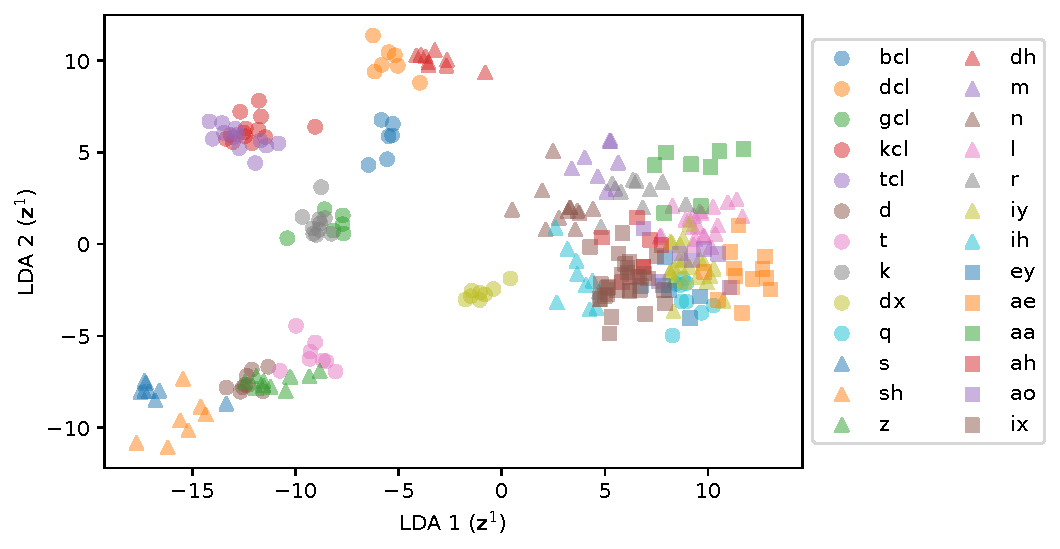
\includegraphics[width=0.555\textwidth]{paper_benchmarking/1xrnjn5y_speaker_phonemes_drw0_latent_0_samples_100_lda_linear_subspace.pdf}
    \hfill
    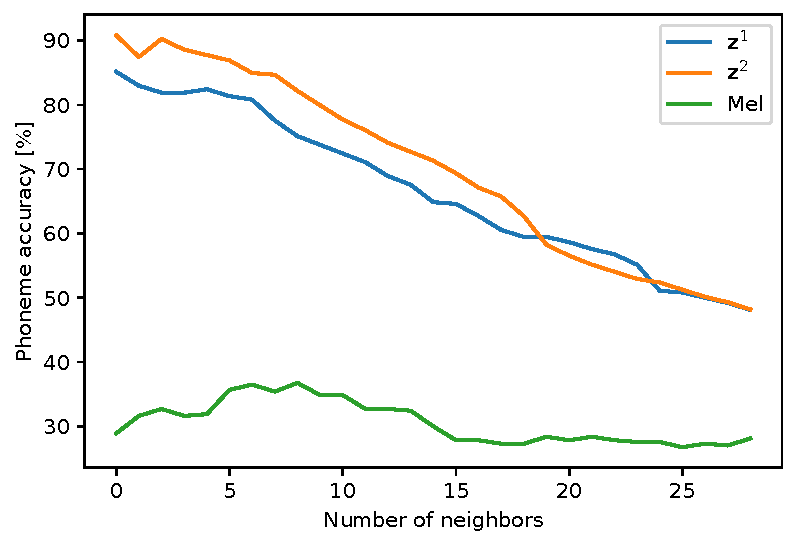
\includegraphics[width=0.425\textwidth]{paper_benchmarking/1xrnjn5y_speaker_phonemes_drw0_samples_100_knn_correct_fraction_model_vs_mel_30_neighbors_lda_subspace_5d.pdf}
    \caption[Clustering of phonemes in 2D subspace of CW-VAE latent space and KNN classification accuracy.]{
    (left) Clustering of phonemes in a 2D Linear Discriminant Analysis (LDA) subspace of a CW-VAE latent space ($\zb^{(1)}$).
    (right) Leave-one-out phoneme classification accuracy for a KNN classifier at different $K$ in a 5D LDA subspace of a CW-VAE latent space.
    }
    \label{fig: latent space phoneme and knn}
\end{figure*}
%

\paragraph{TIMIT}
For temporal resolutions of $s=1$, the deterministic autoregressive models yield the best likelihoods with WaveNet achieving $\SI{10.88}{bpf}$ on TIMIT as seen in \cref{tab: likelihoods timit} (left). 
Somewhat surprisingly, the LSTM baseline almost matches WaveNet with a likelihood of $\SI{11.11}{bpf}$ at $s=1$. However, due to being autoregressive in training, the LSTM trains considerably slower than the parallel convolutional WaveNet; something not conveyed by \cref{tab: likelihoods timit} (left). 
Notably, the VRNN and SRNN models achieve likelihoods close to that of WaveNet and the LSTM at around $\SI{11.09}{bpf}$. The STCN exhibited instability when trained at $s=1$ and tended to diverge.

At $s=64$, WaveNet and the LSTM yield significantly worse likelihoods than all LVMs separated by $\sim\SI{1}{bit}$.
The CW-VAE outperforms the VRNN and SRNN when configured with a hierarchy of latent variables. 
With a single layer of latent variables, the CW-VAE is inferior to both SRNN and VRNN but notably still better than the LSTM. 
These observations carry to $s=256$, where a multilayered CW-VAE outperforms the LSTM, VRNN and SRNN. 
The STCN yields the best results at both $s=64$ and $s=256$. 
For strides $s>1$, previous work has attributed the inferior performance of autoregressive models without latent variables, such as WaveNet and the LSTM, to the ability of LVMs to model intrastep correlations \parencite{lai_re-examination_2019}. 

Decreasing the resolution $s$ improves the likelihood for all LVMs. However, the best performing models, STCN and CW-VAE are not yet scalable to this regime for reasons related to numerical instability and computational infeasibility. This seems to indicate that LVMs may be able to outperform autoregressive models at $s=1$ in the future.
\paragraph{LibriSpeech}
On LibriSpeech (\cref{tab: likelihoods librispeech}), results are similar to TIMIT. The STCN achieves the best likelihood at $s=64$ and the CW-VAE surpasses WaveNet and the LSTM. 
\paragraph{Compression}
A connection can be made between the model likelihoods and the compression rates of audio compression algorithms. 
Lossy compression algorithms, such as MP3, exploit the dynamic range of human hearing to achieve 70-95\% reduction in bit rate \parencite{brandenburg_mpeg-2_1998} while lossless compression algorithms, such as FLAC, achieve 50-70\% reduction \parencite{coalson_free_2019} independent of audio content. 
% On LibriSpeech, FLAC achieves an overall compression to about 58\% of the original bit rate.
Although both the autoregressive models and the LVMs are lossy, their objective minimizes the amount of incurred loss. 
The best likelihoods reported in \cref{tab: likelihoods timit} (left) and \cref{tab: likelihoods librispeech} correspond to about a 30\% reduction in bit rate which indicates that there are significant gains in likelihood to be made in speech modeling.

\section{Phoneme recognition}\label{sec: phoneme recognition}
Although the likelihood is a practical metric for model comparison and selection, a high likelihood does not guarantee that a model has learned useful representations \parencite{huszar_is_2017}. 
For speech data, we would expect models to learn features related to phonetics which would make them useful for tasks such as automatic speech recognition (ASR). 
The Mel spectrogram is a well-established representation of audio designed for speech recognition and is predefined rather than learned. % \parencite{??}. Basic Correlates of the Auditory Stimulus, https://psycnet.apa.org/record/1951-07758-017, modern Mel scale https://ieeexplore.ieee.org/stamp/stamp.jsp?arnumber=1170013&casa_token=UIyQaj3tBRAAAAAA:GtttZedngBkaxVumjnXctc5zS50fptexPMiWhr-7gDrmIVq3JqJPnGCWYedoymb0X5JTGElmHf8&tag=1,
To assess the usefulness of the representations learned by the benchmarked models, we compare them to the highly useful Mel spectrogram on the task of phoneme recognition. 
Phonemes are fundamental units of speech that relate to how parts of words are pronounced (see also appendix~\cref{app: timit phoneme distributions}).
% rather than characters or words themselves (see also appendix~\cref{apsp: timit phoneme distributions}).

\paragraph{Quantitative}
We train an ASR model to recognize phonemes and compare its performance when using input representations obtained from different unsupervised models. 
For WaveNet and the LSTM, we use the hidden state as the representation. For all LVMs, we use the latent variable. For the hierarchical LVMs and WaveNet, we run the experiment using each possible representation and report only the best one here. 
We compare the learned representations to a log Mel spectrogram with 80 filter banks, hop length 64 and window size 128. 
We also compared to using raw PCM in vectors of 64 elements standardized to $[-1,1]$ but found that the ASR did not reliably converge at all which highlights the importance of input representation. 
The ASR model is a three-layered bidirectional LSTM with 256 hidden units. It is trained with the connectionist temporal classification (CTC) loss \parencite{graves_connectionist_2006} which lets it jointly learn to align and classify without using label alignments. 
We pre"=train all unsupervised models at $s=64$ on the full TIMIT training dataset excluding the validation data (3.7h) as in \cref{tab: likelihoods timit} (left). 
We then train the ASR model on all \SI{3.7}{h} as well as \SI{1}{h} and \SI{10}{m} subsets. We report results on the test set in terms of phoneme error rates (PER) in \cref{tab: phoneme recognition (PER)} (right).

As expected, Mel spectrogram performs well achieving 24.1\% PER using 3.7 hours of labeled data. However, the ASR trained on STCN representations outperforms the Mel spectrogram with a PER of 21.9\%. 
This indicates that unsupervised STCN representations are phonetically rich and potentially better suited for speech modeling than the engineered Mel spectrogram. 
When the amount of labeled data is reduced, LVM representations suffer slightly less than deterministic ones. WaveNet representations are interestingly outperformed by both the LSTM and all LVMs. 

% FH-VAE uses 3 layer bidirectional LSTM on 80 mel features. LSTM hidden state dim is 512 or 1024(?)
% FH-VAE https://arxiv.org/pdf/1709.07902.pdf
% [37] https://static.googleusercontent.com/media/research.google.com/da//pubs/archive/43905.pdf
% [13] https://www.cs.toronto.edu/~graves/asru_2013.pdf

\paragraph{Qualitative}
We qualitatively assess the learned latent representations for the CW-VAE. 
We infer the latent variables of all utterances by a single speaker from the TIMIT test set. We sample the latent sequence $100$ times to estimate the mean representation per timestep. We then compute the average latent representation over the duration of each phoneme using aligned phoneme labels. This approximately marginalizes variation during the phoneme. We use linear discriminant analysis (LDA) \parencite{fisher_use_1936} to obtain a low-dimensional linear subspace of the latent space. 
We visualize the resulting representations colored according to test set phoneme classes in \cref{fig: latent space phoneme and knn}. We note that many phonemes are separable in the linear subspace and that related phonemes such as ``s" and ``sh" are close.

We also show the average accuracy of a leave-one-out $k$-nearest-neighbor (KNN) classifier on the single left-out latent representation reduced with a 5-dimensional LDA as a function of the number of neighbors. 
We compare accuracy to a Mel-spectrogram averaged over each phoneme duration and LDA reduced. The spectrogram is computed with hop length set to 64, equal to $s_1$ for the CW-VAE, window size 256 and 80 Mel bins.
We see that both latent spaces yield significantly better KNN accuracies than the Mel features.


\section{Conclusion}
In this paper, we developed a benchmark for speech modeling with stochastic latent variable models (LVMs). 
We compared LVMs and deterministic autoregressive models on equal footing and found that LVMs achieve inferior likelihood compared to deterministic WaveNet and LSTM baselines. Surprisingly, the LSTM almost matched the popular WaveNet model. 
We saw that hierarchical LVMs, such as STCN and CW-VAE, outperformed non-hierarchical versions of themselves in ablation experiments as well as non-hierarchical LVMs such as VRNN and SRNN. This matches recent observations in the image domain. 
We noted that the STCN with an autoregressive decoder outperforms the non"=autoregressive CW-VAE, which we adapted to speech. 
Finally, we found that LVMs can learn latent representations that are useful for phoneme recognition and better than Mel spectrograms, which are tailored for the task, when identical models are trained on top of the representations.
While the best performing models are not yet scalable to the highest temporal resolution, these results indicate that they might improve upon deterministic models in the future. 


%%%%%%%%%%%%%%%%%%%%%%%%%%%%%%%%%%%%%%%%%%%%%%%%%%%%%%%%%%%%%%%%%%%%%%%%%%%%%%%

\section*{Acknowledgements}
This research was partially funded by the Innovation Fund Denmark via the Industrial PhD Programme (grant no.\@ 0153-00167B). JF and SH were funded in part by the Novo Nordisk Foundation (grant no.\@ NNF20OC0062606) via the Center for Basic Machine Learning Research in Life Science (MLLS, \hyperlink{https://www.mlls.dk}{https://www.mlls.dk}). JF was further funded by the Novo Nordisk Foundation (grant no.\@ NNF20OC0065611) and the Independent Research Fund Denmark (grant no.\@ 9131-00082B). SH was further funded by VILLUM FONDEN (15334) and the European Research Council (ERC) under the European Union's Horizon 2020 research and innovation programme (grant agreement no. 757360).

}
